\documentclass[14pt]{beamer}
\setbeamertemplate{caption}[numbered]
\setbeamertemplate{caption label separator}{:}
\setbeamercolor{caption name}{fg=normal text.fg}
\usepackage{amssymb,amsmath}
\usepackage{ifxetex,ifluatex}
\usepackage{fixltx2e} % provides \textsubscript
\usepackage{lmodern}
\ifxetex
  \usepackage{fontspec,xltxtra,xunicode}
  \defaultfontfeatures{Mapping=tex-text,Scale=MatchLowercase}
  \newcommand{\euro}{€}
\else
  \ifluatex
    \usepackage{fontspec}
    \defaultfontfeatures{Mapping=tex-text,Scale=MatchLowercase}
    \newcommand{\euro}{€}
  \else
    \usepackage[T1]{fontenc}
    \usepackage[utf8]{inputenc}
      \fi
\fi
% use upquote if available, for straight quotes in verbatim environments
\IfFileExists{upquote.sty}{\usepackage{upquote}}{}
% use microtype if available
\IfFileExists{microtype.sty}{\usepackage{microtype}}{}
\PassOptionsToPackage{hyphens}{url}
\usepackage{hyperref}
\usepackage{ulem}

% Comment these out if you don't want a slide with just the
% part/section/subsection/subsubsection title:
\AtBeginPart{
  \let\insertpartnumber\relax
  \let\partname\relax
  \frame{\partpage}
}
\AtBeginSection{
  \let\insertsectionnumber\relax
  \let\sectionname\relax
  \begin{frame}[plain]
    \tableofcontents[currentsection]
  \end{frame}
}
\AtBeginSubsection{
  \let\insertsubsectionnumber\relax
  \let\subsectionname\relax
  \frame{\subsectionpage}
}

\setlength{\parindent}{0pt}
\setlength{\parskip}{6pt plus 2pt minus 1pt}
\setlength{\emergencystretch}{3em}  % prevent overfull lines
\setcounter{secnumdepth}{0}
% Thanks Richard Darst on how to get a nice Beamer theme.
% See http://rkd.zgib.net/wiki/DebianBeamerThemes

\usepackage{multicol}
\usepackage{tikz}
\usepackage{ctable}
\usetikzlibrary{positioning}

\usebackgroundtemplate{
\includegraphics[width=\paperwidth]{images/swirl-lightest.pdf}}
\logo{
\includegraphics[viewport=274 335 360 440,width=1cm]{images/openlogo-nd.pdf}}

\definecolor{debianred}{rgb}{.780,.000,.211} % 199,0,54
\definecolor{debianblue}{rgb}{0,.208,.780} % 0,53,199
\definecolor{debianlightbackgroundblue}{rgb}{.941,.941,.957} % 240,240,244
\definecolor{debianbackgroundblue}{rgb}{.776,.784,.878} % 198,200,224

\usetheme{Boadilla}
\setbeamertemplate{navigation symbols}{}

\usecolortheme[named=debianbackgroundblue]{structure}
\setbeamercolor{normal text}{fg=black}
\setbeamercolor{titlelike}{fg=debianblue}
\setbeamercolor{sidebar}{fg=debianred,bg=debianbackgroundblue}

\setbeamercolor{palette sidebar primary}{fg=debianred}
\setbeamercolor{palette sidebar secondary}{fg=debianred}
\setbeamercolor{palette sidebar tertiary}{fg=debianred}
\setbeamercolor{palette sidebar quaternary}{fg=debianred}

\setbeamercolor{section in toc}{fg=debianred}
\setbeamercolor{subsection in toc}{parent=debianred}

\setbeamercolor{item}{fg=debianred}

\setbeamercolor{block title}{fg=debianblue}

\title[Reproducible builds]{Beyond reproducible builds}
\subtitle{We are not there yet and why \\ "just" achieving reproducible builds
\\ won't be enough}
\author[lamby \& h01ger]{%
   \texorpdfstring{
        \begin{columns}
            \column{.45\linewidth}
            \centering
            Chris Lamb (lamby) \\
            \href{mailto:lamby@debian.org}{lamby@debian.org}
            \column{.45\linewidth}
            \centering
            Holger 'h01ger' Levsen\\
            \href{mailto:holger@debian.org}{holger@debian.org}
        \end{columns}
   }{lamby \& h01ger}}
\institute[Debian]{}
\date[MiniDebConf Cambridge '15]{%
 MiniDebConf 2015\\
 Cambridge, UK\\
 2015-11-06}

\begin{document}

\begin{frame}
 \titlepage
\end{frame}

\begin{frame}
 \frametitle{Debian reproducible builds team}
 \begin{center}
  \begin{columns}
   \small
   \column{.33\linewidth}
    {akira} \\
    {Andrew Ayer} \\
    {Asheesh Laroia} \\
    \only<1>{Chris Lamb}\only<2>{{\color{debianblue} Chris Lamb}} \\
    {Chris West} \\
    {Christoph Berg} \\
    {Daniel Kahn Gillmor} \\
    David Suarez \\
    {Dhole} \\
    Drew Fisher \\
    Esa Peuha \\
    {Guillem Jover} \\
   \column{.33\linewidth}
    Hans-Christoph Steiner \\
    {Helmut Grohne} \\
    \only<1>{Holger Levsen}\only<2>{{\color{debianblue} Holger Levsen}} \\
    Jelmer Vernooij \\
    {josch} \\
    Juan Picca \\
    {Lunar} \\
    Mathieu Bridon \\
    {Mattia Rizzolo} \\
    Nicolas Boulenguez \\
    {Niels Thykier} \\
    Niko Tyni \\
   \column{.33\linewidth}
    {Paul Wise} \\
    Peter De Wachter \\
    Philip Rinn \\
    {Reiner Herrmann} \\
    {Stefano Rivera} \\
    {Stéphane Glondu} \\
    {Steven Chamberlain} \\
    Tom Fitzhenry \\
    Valentin Lorentz \\
    {Wookey} \\
    {Ximin Luo} \\
  \end{columns}
 \end{center}
\end{frame}

\begin{frame}
 \frametitle{Who are you?}
 \begin{itemize}
  \item Who has seen a previous talk about reproducible builds this year?
  \item<2-3> Who has contributed to this effort already?
  \item<3> Who thinks "packages \textbf{should} produce reproducible binaries"
    should be added to policy now?
 \end{itemize}
\end{frame}

\section{About}

\begin{frame}
 \frametitle{In-depth explaination of the problem}

 \begin{center}
  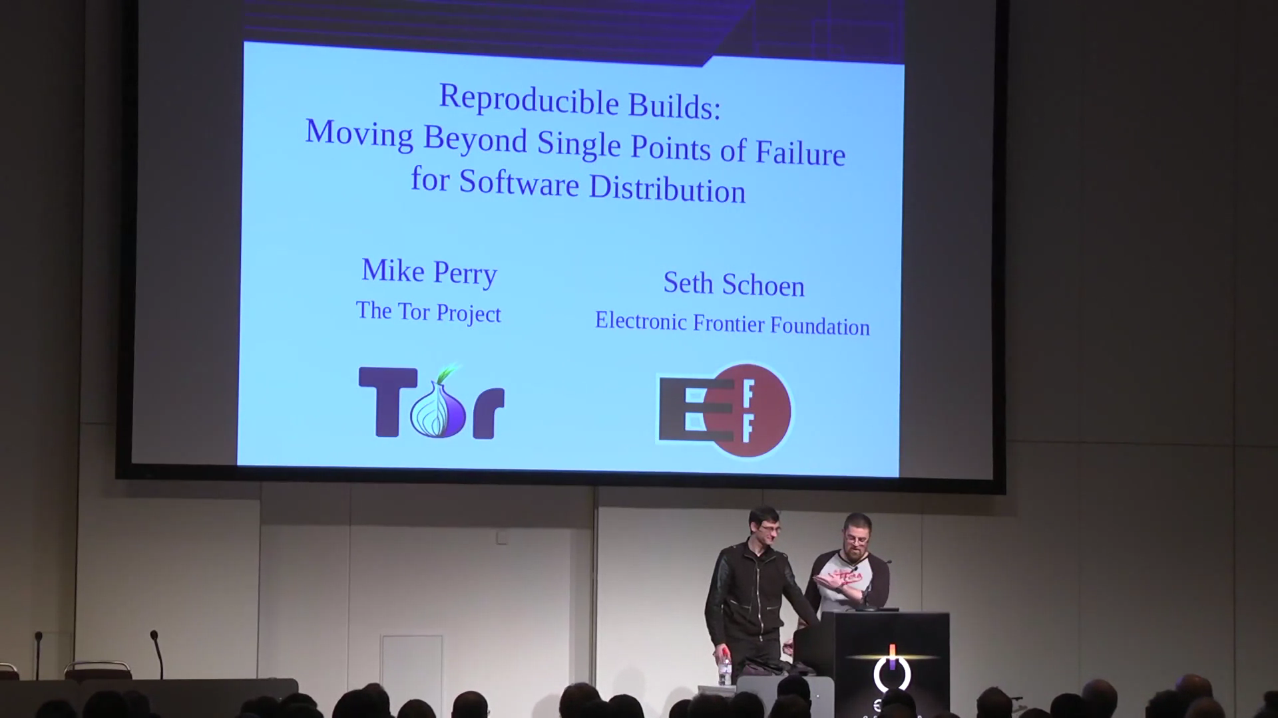
\includegraphics[width=0.7\textwidth]{images/31c3.png}

  Available on \url{media.ccc.de}, 31c3
 \end{center}
\end{frame}

\begin{frame}
 \frametitle{The solution}

 \begin{center}
 \Large{
 enable anyone to reproduce
 identical binary packages
 from a given source}
\end{center}
\end{frame}


\begin{frame}
 \frametitle{A little demo}

  make, make, diff
  make, make, diff
  make, make, diff
\end{frame}


\begin{frame}
 \frametitle{The solution}

 \begin{center}
 We call this:

 \Huge{ “reproducible builds” }
 \end{center}
\end{frame}


\begin{frame}[plain]
\begin{center}
 \Huge{It should become the \textbf{norm}.}

 \visible<2>{\small{ We want to change the meaning of "free software":

  it's only free software if it is reproducible!}}
\end{center}
\end{frame}

\section{Status in Debian}

\begin{frame}[plain]
 \frametitle{Progress in Debian \texttt{unstable}}
 \begin{center}
  \includegraphics[height=0.5\paperheight]{images/stats_pkg_state.png}

  \small{19500 out of 23079 source packages are reproducible \\
    in our current test framework}
  \vfill
 \end{center}
\end{frame}


\begin{frame}[plain]
 \frametitle{Progress in the Debian BTS}
 \begin{tikzpicture}[remember picture,overlay]
  \node[at=(current page.center)] {
    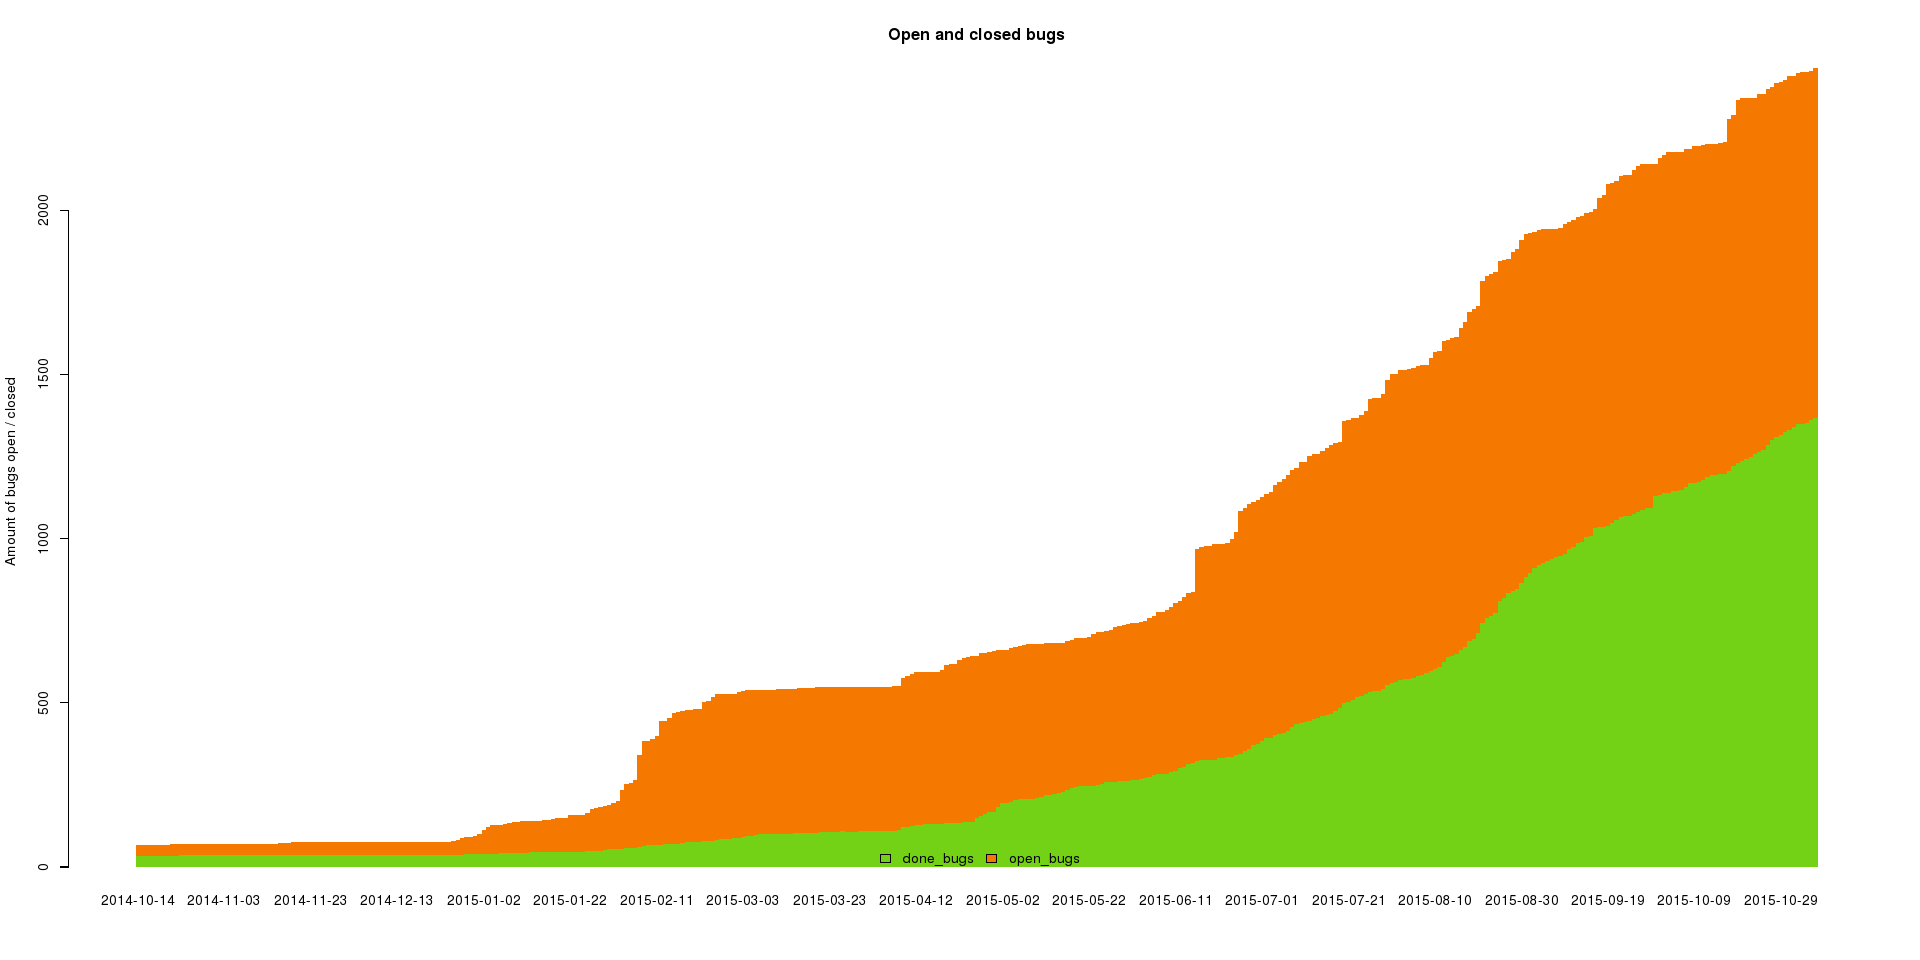
\includegraphics[width=\paperwidth]{images/stats_bugs_state.png}
  };
 \end{tikzpicture}
\end{frame}


\begin{frame}
 \frametitle{What we did since Summer 2014}

 \begin{itemize}
  \item Agreed on using a fixed build path: \texttt{/build}
  \item Record the build environment: \texttt{.buildinfo}
  \item \texttt{strip-nondeterminism}
  \item \texttt{reproducible.debian.net}
  \item \texttt{diffoscope} (formerly known as \texttt{debbindiff})
  \item \texttt{SOURCE\_DATE\_EPOCH}
  \item \texttt{disorderfs}
  \item Over 700 patches: \texttt{dpkg}, \texttt{debhelper}, \texttt{sbuild}, …
  \item<2> Tell the world \& collaborate
 \end{itemize}
\end{frame}

\begin{frame}
 \frametitle{Tell the world \& collaborate}

 \begin{itemize}
  \item Two recent talks available with subtitles:
   \begin{itemize}
    \item 2015-08-13: Chaos Communication Camp 2015
    \item 2015-08-20: DebConf15
   \end{itemize}
  \item Weekly reports since May 2015
  \item Summit in December 2015 in Athens
   \begin{itemize}
    \item 40 people from 16 projects
   \end{itemize}
 \end{itemize}
\end{frame}

\begin{frame}
 \frametitle{Tell the world \& collaborate, cont.}

 \begin{center}
 \texttt{https://reproducible-builds.org}

 
\includegraphics[width=0.7\textwidth]{images/rbwww1.png}
 \end{center}
\end{frame}

\begin{frame}
 \frametitle{Update on reproducible.debian.net}

 \begin{itemize}
  \item maintained in \texttt{jenkins.debian.net.git} by 27 contributors
  \item \small{4k lines of Python and 5k lines Bash code run by 111 jenkins
  now running on 10 hosts}
  \item Continuously testing Debian testing, unstable and experimental
  \item Not just testing Debian, but also Coreboot, OpenWrt, NetBSD, FreeBSD,
  Archlinux and soon Fedora
  \item \texttt{amd64}: 109 cores and 194 GB RAM split on 8 VMs, provided by ProfitBricks.
  \item \texttt{armhf}: 12 cores and 6 GB RAM on 4 systems, provided by
  Vagrant@d.o.
 \end{itemize}
 \vfill
 \begin{center}
 
\includegraphics[height=0.15\paperheight]{images/profitbricks_logo.png}
 \end{center}
\end{frame}

\begin{frame}
 \frametitle{Future of reproducible.debian.net}

 \begin{itemize}
 \item We want more more more arm(64) cores!
 \item ...
 \begin{center}
  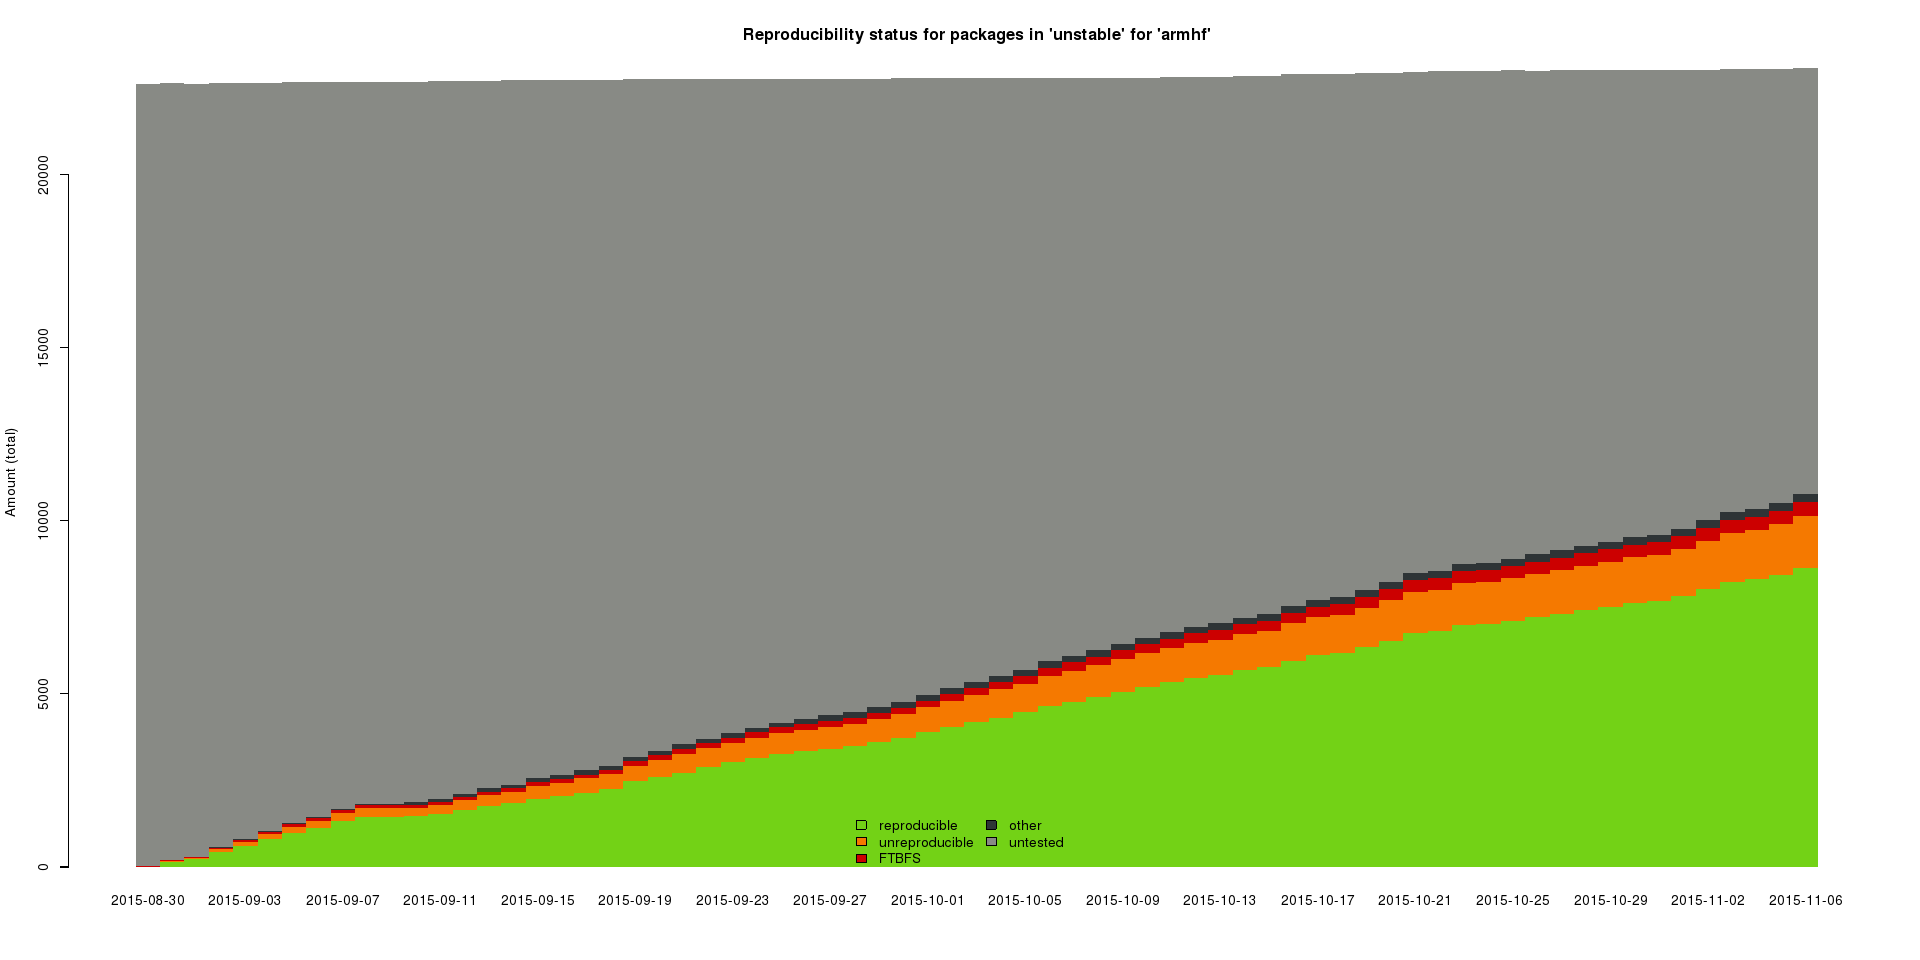
\includegraphics[height=0.5\paperheight]{images/stats_pkg_state_armhf.png}
  \vfill
 \end{center}
 \end{itemize}
\end{frame}


\begin{frame}[fragile]
 \frametitle{Variations on reproducible.debian.net}

 \begin{center}
  \begin{table}
   \resizebox{0.95\textwidth}{!}{%
    \begin{tabular}{l|ll}
\textbf{variation} & \textbf{first build} & \textbf{second build} \\
\hline
hostname & \texttt{jenkins} & \texttt{i-capture-the-hostname} \\
domainname & \texttt{debian.net} & \texttt{i-capture-the-domainname} \\
\texttt{env TZ} & \texttt{GMT+12} & \texttt{GMT-14} \\
\texttt{env LANG} & \texttt{en\_GB.UTF-8} & \texttt{fr\_CH.UTF-8} \\
\texttt{env LC\_ALL} & not set & \texttt{fr\_CH.UTF-8} \\
\texttt{env USER} & \texttt{pbuilder1} & \texttt{pbuilder2} \\
uid & \texttt{1111} & \texttt{2222} \\
gid & \texttt{1111} & \texttt{2222} \\
UTS namespace & shared with the host & \textit{modified using \texttt{/usr/bin/unshare --uts}} \\
kernel version & Linux 3.16.0-4-amd64 & Linux 2.6.56-4-amd64 \\
umask & 0022 & 0002 \\
CPU type & \multicolumn{2}{l}{same for both builds \textit{(work in progress)}} \\
filesystem & \multicolumn{2}{l}{same for both builds \textit{(work in progress - disorderfs)}} \\
year, month, date & \multicolumn{2}{l}{same for both builds \textit{(work in progress)}} \\
hour, minute & \multicolumn{2}{l}{hour is usually the same… usually, the minute differs… \textit{(work in progress)}} \\
\textit{everything else} & \multicolumn{2}{l}{\textit{is likely the same…}}
    \end{tabular}
   }
  \end{table}
 \end{center}
\end{frame}



\begin{frame}
 \frametitle{Debian .buildinfo}

 \begin{itemize}
  \item Aggregate in the same file:
   \begin{itemize}
    \item Sources (checksums)
    \item Generated binaries (checksums)
    \item Packages used to build (with specific version, checksums coming soon)
   \end{itemize}
  \item Can be later used to reinstall environment exactly as it was
  \item For Debian, all versions are available from \url{snapshot.debian.org}
 \end{itemize}
\end{frame}


\begin{frame}[fragile]
 \frametitle{Example .buildinfo}

{\small
\begin{verbatim}
Format: 1.9
Build-Architecture: amd64
Source: txtorcon
Binary: python-txtorcon
Architecture: all
Version: 0.11.0-1
Build-Path: /buildd/debian/txtorcon-0.11.0-1
Checksums-Sha256:
 a26549d9…7b 125910 python-txtorcon_0.11.0-1_all.deb
 28f6bcbe…69 2039 txtorcon_0.11.0-1.dsc
Build-Environment:
 base-files (= 8),
 base-passwd (= 3.5.37),
 bash (= 4.3-11+b1),
 …
\end{verbatim}
}
\end{frame}



{
\usebackgroundtemplate{%
 \begin{tikzpicture}[remember picture,overlay]%
  \node[shift={(-0.15\paperwidth, 0.4\paperheight)},at=(current page.south east)] {
    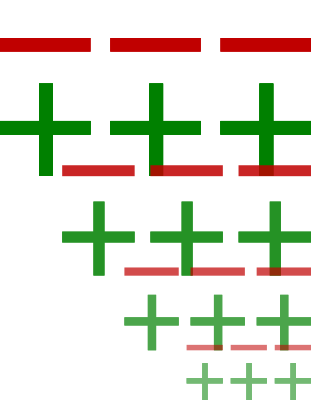
\includegraphics[width=0.2\paperwidth]{images/diffoscope_logo.png}
  };
 \end{tikzpicture}%
}
\begin{frame}{diffoscope}
 \frametitle{Debugging problems: diffoscope}

 \begin{itemize}
  \item Examines differences \textbf{in depth}
  \item Outputs HTML or plain text showing the differences
  \item Recursively unpacks archives
  \item Seeks human readability:
   \begin{itemize}
    \item uncompresses PDF
    \item disassembles binaries
    \item unpacks Gettext files
    \item … \textit{easy to extend to new file formats}
   \end{itemize}
  \item Falls back to binary comparison
  \item Available in Debian sid and stretch
  \item Maintainers in other distros wanted
 \end{itemize}
 \vfill
 \begin{center}
  \url{http://diffoscope.org/}\\
  {\footnotesize \color{gray}{(formely known as \texttt{debbindiff})}}
 \end{center}
\end{frame}
}

\begin{frame}
 \frametitle{diffoscope example (HTML output)}

 \begin{center}
  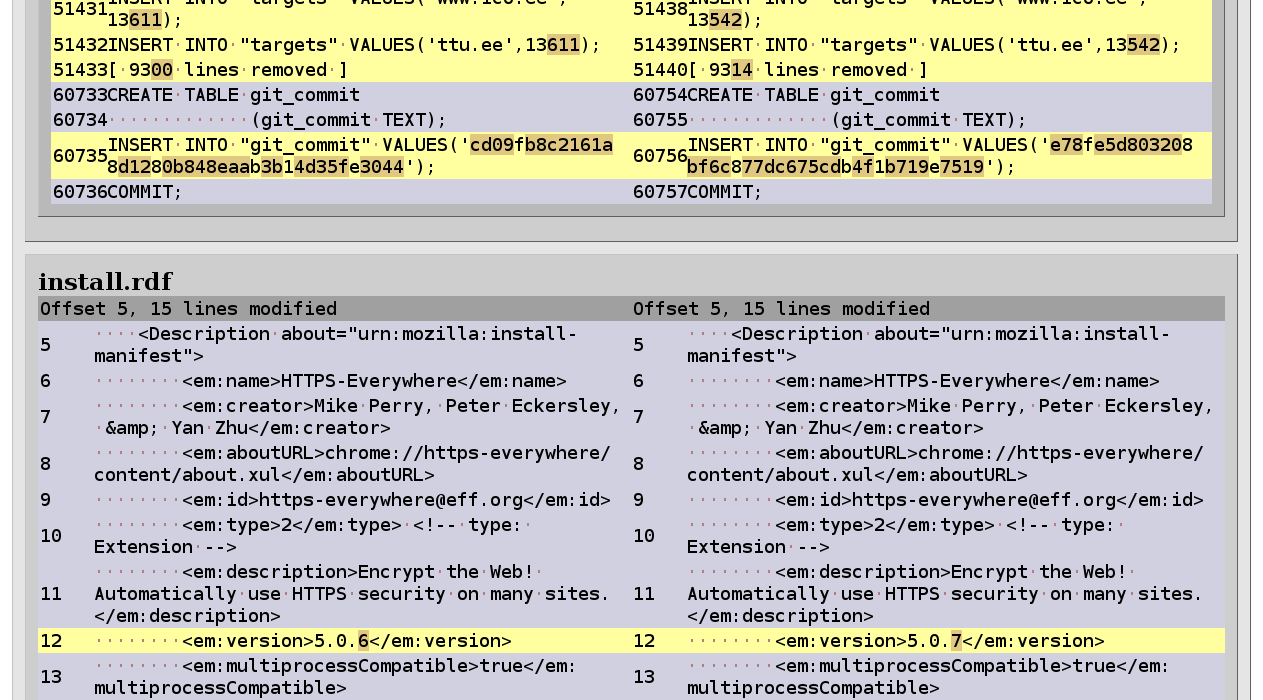
\includegraphics[width=0.9\paperwidth]{images/diffoscope_example_html.png}
 \end{center}
\end{frame}

\begin{frame}
 \frametitle{\texttt{diffoscope} is "just" for debugging}

 \begin{itemize}
  \item Reminder: \texttt{diffoscope} is for \textbf{debugging}
  \item<2> "reproducible" according to our definition means: \textbf{bit by bit
  identical}. So the tools for testing whether something is reproducible are
  either \texttt{diff} or \texttt{sha256sum}!
 \end{itemize}
\end{frame}


\begin{frame}
 \frametitle{\texttt{SOURCE\_DATE\_EPOCH}}

 \begin{itemize}
  \item Build date usually not useful for the user
  \item Standardize a build-time environment variable
  \item Value of \texttt{SOURCE\_DATE\_EPOCH} is used instead of the current date
  \item General solution for other free software projects and distributions
  \item In Debian, set from the latest \texttt{debian/changelog} entry
 \end{itemize}
\end{frame}

\begin{frame}
 \frametitle{\texttt{SOURCE\_DATE\_EPOCH} (closed bugs)}

 \begin{itemize}
  \item \sout{\texttt{\#791823}}: debhelper
  \item \sout{\texttt{\#787444}}: help2man
  \item \sout{\texttt{\#790899}}: epydoc
  \item \sout{\texttt{\#794004}}: ghostscript
  \item \sout{\texttt{\#783475}}: texi2html
  \item \sout{\texttt{\#794586}}: ocamldoc
  \item sphinx \small{\url{https://github.com/sphinx-doc/sphinx/pull/1954}}
 \end{itemize}

\end{frame}

\begin{frame}
 \frametitle{\texttt{SOURCE\_DATE\_EPOCH} (open bugs)}

 \begin{itemize}
  \item gcc (\texttt{\_\_DATE\_\_} and \texttt{\_\_TIME\_\_} macros) \texttt{\footnotesize{\url{https://gcc.gnu.org/ml/gcc-patches/2015-06/msg02210.html}}}
  \item \texttt{\#792687}: gettext (xgettext)
  \item \texttt{\#792201}: doxygen
  \item \texttt{\#800797}: docbook-utils
  \item \texttt{\#790801}: txt2man
  \item \texttt{\#791815}: libxslt
  \item \texttt{\#794681}: qt4-x11 (qthelpgenerator)
  \item \texttt{\#792202}: texlive-bin
 \end{itemize}

\end{frame}


\section{Missing bits}

\begin{frame}
 \frametitle{Status and next steps in Debian}
 \begin{itemize}
  \item Remember: this is just a proof-of-concept, Debian is not 80\%
  reproducible.
  \item Major changes still need to be merged.
  \item Once this has happend, Debian will be >80\% reproducible.
  \item The next Debian release ("stretch") shall be >80\% reproducible.
 \end{itemize}
\end{frame}

\begin{frame}
 \frametitle{dpkg}

 \begin{itemize}\small
  \item \sout{\texttt{\#719844}: make compression of \{data,control\}.tar.gz deterministic}
  \item \texttt{\#759999}: set reproducible timestamps in \texttt{.deb} ar file headers
  \item \texttt{\#787980}: normalize file permissions when creating control.tar
  \item \texttt{\#719845}: make file order within {data,control}.tar.gz deterministic
  \item \texttt{dpkg-genbuldinfo}: \textit{patch already written, but waiting on agreement about spec}
 \end{itemize}
\end{frame}

\begin{frame}
 \frametitle{debhelper}

 \begin{itemize}\small
  \item \texttt{\#759886}: make mtimes of packaged files deterministic
  \item \sout{\texttt{\#759895}: add a call to
  \texttt{dh\_strip\_nondeterminism} in \texttt{dh}}
  \item \sout{\texttt{\#791823}: set \texttt{SOURCE\_DATE\_EPOCH} env var for
  reproducible builds}
 \end{itemize}
\end{frame}

\begin{frame}
 \frametitle{sbuild}

 \begin{itemize}\small
  \item \sout{\texttt{\#790868}: allow sbuild to use a deterministic build
  path to build packages}
  \item \texttt{\#778571}: predictible build location for reproducible builds
  \item Finish the \texttt{srebuild} script
 \end{itemize}
\end{frame}

\begin{frame}
 \frametitle{ftp.debian.org}

 \begin{itemize}\small
  \item \texttt{\#763822}: please include .buildinfo file in the archive
 \end{itemize}
\end{frame}

\begin{frame}
 \frametitle{"Finally", changing Debian policy}

 \begin{itemize}
  \item Section 4.15: “Sources \textbf{must} build reproducible binaries.”
  \item<2-3> We hope this will happen in early 2017 = after the Stretch
  (Debian 9) release
  \item<3> in 2016, hopefully: “Sources \textbf{shall} build reproducible binaries.”
 \end{itemize}
\end{frame}

\section{Beyond builds}

\begin{frame}
 \frametitle{Reproducible builds demand a defined build environment}
 \begin{itemize}
  \item Re-creating an identical build environment is mandatory too.
  \item Without an identical build environment reproducible builds will only happen by sheer luck, thus that's not really reproducible at all.
  \item<2>{This is probably only solved for Debian right now - and currently that's still a proof of concept only…}
 \end{itemize}
\end{frame}

\begin{frame}
 \frametitle{Reproducible builds are just the first step}
 \begin{itemize}
  \item Continuous rebuilds need to happen in a systematic way and the resulting checksums need to be properly published.
  \item<2> Integration in end user tools\\
  "Do you really want to install this unreproducible software (y/N)"\\
  "Which rebuilders do you want to trust?"
 \end{itemize}
\end{frame}

\begin{frame}
 \frametitle{Status of reproducible builds in other distros}

 \begin{itemize}
  \item As shown we're also testing Coreboot, OpenWrt, NetBSD, FreeBSD, Archlinux and soon Fedora.
  \item But the work needs to be done within those projects.
  \item<2> And we are only testing for reproducible builds. No work has been done on the other 66\% yet. (Systematic rebuilds and sharing the checksum \& end-user tool integration)
 \end{itemize}
\end{frame}


\section{Want to help?}

\begin{frame}
 \frametitle{As a software developer}
 \begin{itemize}
  \item stop using build dates
  \item use \texttt{SOURCE\_DATE\_EPOCH} instead
  \item see \url{https://reproducible-builds.org/specs/}
 \end{itemize}
\end{frame}

\begin{frame}
 \frametitle{Get involved - learning by doing}

 \begin{itemize}
  \item Test for yourself:
   \begin{itemize}
    \item just build something twice, run diffoscope on the results
    \begin{itemize}
     \item for better results use our “reproducible” repository, \texttt{pbuilder} and a custom config
    \end{itemize}
   \end{itemize}
  \item Tips on the wiki: \\
    \small{\url{https://wiki.debian.org/ReproducibleBuilds/Howto}} \\
    \small{\url{https://wiki.debian.org/ReproducibleBuilds/ExperimentalToolchain}}
  \item Ask for help on \texttt{\#debian-reproducible} or on the mailing-list
 \end{itemize}
\end{frame}

\begin{frame}
 \frametitle{Join the team!}

 \begin{itemize}
  \item Why?
   \begin{itemize}
    \item \heartsuit{}\heartsuit{}\heartsuit{} Lovely group of people \heartsuit{}\heartsuit{}\heartsuit{}
    \item Learn something new everyday
    \item Change the (software) world!
   \end{itemize}
  \item What do we do?
   \begin{itemize}
    \item Review packages
    \item Identify issues and document solutions
    \item \texttt{reproducible.d.n}, diffoscope, strip-nondeterminism
    \item Propose changes for toolchain
    \item Submit patches for individual packages
    \item Write more general documentation and talk to the world
   \end{itemize}
 \end{itemize}
\end{frame}

\begin{frame}
 \frametitle{Write a thesis!}

 \begin{itemize}
  \item We are trying to document all our work, but we won't write scientific articles.
  \item Maybe you can do that?
 \end{itemize}
\end{frame}


\section{Questions, comments, ideas?}


\begin{frame}
 \frametitle{Questions, comments, ideas?}

 \begin{itemize}
  \item \url{https://reproducible-builds.org}
  \item \url{https://reproducible.debian.net}
  \item \href{mailto:reproducible-builds@lists.alioth.debian.org}{reproducible-builds@lists.alioth.debian.org}
  \item \texttt{\#debian-reproducible} on \texttt{irc.OFTC.net}
 \end{itemize}
\end{frame}


\begin{frame}
 \frametitle{Thanks!}

 \begin{itemize}
  \item Debian “Reproducible Builds” team \\
        {\small (you are just \textbf{so} awesome!)}
  \item Linux Foundation and the Core Infrastructure Initiative
  \item MiniDebConf Cambridge 2015
\end{itemize}

 \begin{center}
  
\includegraphics[height=0.1\paperheight]{images/linux_foundation_logo.png}
  \hspace{0.1\paperwidth}
  
\includegraphics[height=0.1\paperheight]{images/cii_logo.png}
 \end{center}

 \vfill
 \begin{center}
  \resizebox{0.8\textwidth}{!}{%
   \begin{tabular}{rl}
    \texttt{holger@debian.org} & \texttt{B8BF 5413 7B09 D35C F026} \\
                               & \texttt{FE9D 091A B856 069A AA1C} \\
    \texttt{lamby@debian.org} & \texttt{C2FE 4BD2 71C1 39B8 6C53} \\
                              & \texttt{3E46 1E95 3E27 D431 1E58}
   \end{tabular}
  }
 \end{center}
\end{frame}

\end{document}
